\documentclass[11pt,ngerman,a4paper,]{article}
\usepackage{lmodern}

\usepackage{amssymb,amsmath}
\usepackage{tikz}
\usepackage{float}

\usepackage{enumitem}
\newlist{todolist}{itemize}{2}
\setlist[todolist]{label=$\square$}

\usepackage{ifxetex,ifluatex}
\usepackage{fixltx2e} % provides \textsubscript
\ifnum 0\ifxetex 1\fi\ifluatex 1\fi=0 % if pdftex
  \usepackage[T1]{fontenc}
  \usepackage[utf8]{inputenc}
\else % if luatex or xelatex
  \usepackage{unicode-math}
  \defaultfontfeatures{Ligatures=TeX,Scale=MatchLowercase}
\fi
% use upquote if available, for straight quotes in verbatim environments
\IfFileExists{upquote.sty}{\usepackage{upquote}}{}
% use microtype if available
\IfFileExists{microtype.sty}{%
\usepackage[]{microtype}
\UseMicrotypeSet[protrusion]{basicmath} % disable protrusion for tt fonts
}{}
\PassOptionsToPackage{hyphens}{url} % url is loaded by hyperref
\usepackage[unicode=true]{hyperref}
\hypersetup{
            pdftitle={Vorhersage der Stromerzeugung basierend auf Self Learning Activation Functions und Liquid Neuronal Networks},
            pdfkeywords={SLAF, LNN, Forecasting},
            pdfborder={0 0 0},
            breaklinks=true}
\urlstyle{same}  % don't use monospace font for urls
\usepackage{geometry}
\geometry{left=2.5cm,right=2.5cm,top=2.5cm,bottom=2.5cm}
\ifnum 0\ifxetex 1\fi\ifluatex 1\fi=0 % if pdftex
  \usepackage[shorthands=off,main=ngerman]{babel}
\else
  \usepackage{polyglossia}
  \setmainlanguage[]{}
\fi
\usepackage[style=authoryear-comp,]{biblatex}
\addbibresource{references.bib}
\usepackage{longtable,booktabs}
% Fix footnotes in tables (requires footnote package)
\IfFileExists{footnote.sty}{\usepackage{footnote}\makesavenoteenv{long table}}{}

\usepackage{graphicx,grffile}
\makeatletter
\def\maxwidth{\ifdim\Gin@nat@width>\linewidth\linewidth\else\Gin@nat@width\fi}
\def\maxheight{\ifdim\Gin@nat@height>\textheight\textheight\else\Gin@nat@height\fi}
\makeatother
% Scale images if necessary, so that they will not overflow the page
% margins by default, and it is still possible to overwrite the defaults
% using explicit options in \includegraphics[width, height, ...]{}
\setkeys{Gin}{width=\maxwidth,height=\maxheight,keepaspectratio}
\IfFileExists{parskip.sty}{%
\usepackage{parskip}
}{% else
\setlength{\parindent}{0pt}
\setlength{\parskip}{6pt plus 2pt minus 1pt}
}
\setlength{\emergencystretch}{3em}  % prevent overfull lines
\providecommand{\tightlist}{%
  \setlength{\itemsep}{0pt}\setlength{\parskip}{0pt}}
\setcounter{secnumdepth}{5}

% set default figure placement to htbp
\makeatletter
\def\fps@figure{htbp}
\makeatother


\title{Vorhersage der Stromerzeugung basierend auf Self Learning Activation Functions und Liquid Neuronal Networks}

%% MONASH STUFF

%% CAPTIONS
\RequirePackage{caption}
\DeclareCaptionStyle{italic}[justification=centering]
 {labelfont={bf},textfont={it},labelsep=colon}
\captionsetup[figure]{style=italic,format=hang,singlelinecheck=true}
\captionsetup[table]{style=italic,format=hang,singlelinecheck=true}

%% FONT
\RequirePackage{bera}
\RequirePackage{mathpazo}

%% HEADERS AND FOOTERS
\RequirePackage{fancyhdr}
\pagestyle{fancy}
\rfoot{\Large\sffamily\raisebox{-0.1cm}{\textbf{\thepage}}}
\makeatletter
\lhead{\textsf{\expandafter{\@title}}}
\makeatother
\rhead{}
\cfoot{}
\setlength{\headheight}{15pt}
\renewcommand{\headrulewidth}{0.4pt}
\renewcommand{\footrulewidth}{0.4pt}
\fancypagestyle{plain}{%
\fancyhf{} % clear all header and footer fields
\fancyfoot[C]{\sffamily\thepage} % except the center
\renewcommand{\headrulewidth}{0pt}
\renewcommand{\footrulewidth}{0pt}}

%% MATHS
\RequirePackage{bm,amsmath}
\allowdisplaybreaks

%% GRAPHICS
\RequirePackage{graphicx}
\setcounter{topnumber}{2}
\setcounter{bottomnumber}{2}
\setcounter{totalnumber}{4}
\renewcommand{\topfraction}{0.85}
\renewcommand{\bottomfraction}{0.85}
\renewcommand{\textfraction}{0.15}
\renewcommand{\floatpagefraction}{0.8}

%\RequirePackage[section]{placeins}

%% SECTION TITLES
\RequirePackage[compact,sf,bf]{titlesec}
\titleformat{\section}[block]
  {\fontsize{15}{17}\bfseries\sffamily}
  {\thesection}
  {0.4em}{}
\titleformat{\subsection}[block]
  {\fontsize{12}{14}\bfseries\sffamily}
  {\thesubsection}
  {0.4em}{}
\titlespacing{\section}{0pt}{*5}{*1}
\titlespacing{\subsection}{0pt}{*2}{*0.2}


%% TITLE PAGE
\def\Date{\number\day}
\def\Month{\ifcase\month\or
 January\or February\or March\or April\or May\or June\or
 July\or August\or September\or October\or November\or December\fi}
\def\Year{\number\year}

\makeatletter
\def\wp#1{\gdef\@wp{#1}}\def\@wp{??/??}
\def\jel#1{\gdef\@jel{#1}}\def\@jel{??}
\def\showjel{{\large\textsf{\textbf{JEL classification:}}~\@jel}}
\def\nojel{\def\showjel{}}
\def\addresses#1{\gdef\@addresses{#1}}\def\@addresses{??}
\def\cover{{\sffamily\setcounter{page}{0}
        \thispagestyle{empty}
        \placefig{2}{1.5}{width=5cm}{FHSWF}
        %\placefig{16.9}{1.5}{width=2.1cm}{MBusSchool}
        %\begin{textblock}{4}(16.9,4)ISSN 1440-771X\end{textblock}
        \begin{textblock}{7}(12.7,27.9)\hfill
        
\includegraphics[height=1cm]{WirGebenImpulse}~~~
        %\includegraphics[height=0.7cm]{EQUIS}~~~
        %\includegraphics[height=0.7cm]{AMBA}
        \end{textblock}
        \vspace*{0.5cm}
        \begin{center}\Large
                  Fachhochschule Südwestfalen\\
          Fachbereich Ingenieur- und Wirtschaftswissenschaften\\[.5cm]
                %%
         Neuronal Network and Deep Learning (Prof.~Dr.~Thomas Kopinski und Felix Neubürger) \\ 
        \normalsize   Gutachter: Prof.~Dr.~Thomas Kopinski und Felix Neubürger   
        %%
        \end{center}\vspace{1cm}
        \begin{center}
        \fbox{\parbox{14cm}{\begin{onehalfspace}\centering\huge\vspace*{0.2cm}
                \textsf{\textbf{\expandafter{\@title}}}\vspace{1cm}\par
                \LARGE\@author\end{onehalfspace}
        }}
        %%
        %%
        \end{center}
        %%
        \vspace{2cm}
                \begin{singlespace}
        \begin{abstract}
        \footnotesize
        Bei der Vorhersage von Zeitreihen kann die Anpassung an die aktuelle Situation eine große Rolle spielen. So i.d.r. ob z.B. Umwelteinflüsse oder Pandemien eine große Veränderung in einer Zeitreihe herbeiführen. Der erste Ansatz für eine Vorhersage von Zeitreihen basiert in dieser Arbeit auf den Liquid Neuronal Networks (LNN). Die LNNs sind dynamisch und passen sich an die aktuelle Situation an, lernen also immer weiter. Als eine Ergänzung zu den LNNs wir die Self Learning Activation Function (SLAF) implementiert. Diese approximiert die Parametrierung der richtigen Aktivierungsfunktion. Das Neuronale Netz wird auf den Datensatz der Stromerzeugung in den Jahren 2004-2018 vom Unternehmen American Electric Power angewandt.
        \end{abstract}
        \end{singlespace}
                        \begin{keywords}
        \footnotesize
        SLAF, LNN, Forecasting
        \end{keywords}
                %%
        \vfill
                \begin{center}
                \footnotesize
                Meschede\linebreak
                \today
        \end{center}\vspace*{0.5cm}}}
\def\pageone{{\sffamily\setstretch{1}%
        \thispagestyle{empty}%
        \vbox to \textheight{%
                {\fontsize{24.88}{30}\sffamily\textbf{\expandafter{Ehrenwörtliche Erklärung}}}
        \vspace{1cm}\par
        Ich erkläre hiermit ehrenwörtlich, dass ich die vorliegende Arbeit selbständig angefertigt habe. Die aus fremden Quellen direkt und indirekt übernommenen Gedanken sind als solche kenntlich gemacht. Die Arbeit wurde weder einer anderen Prüfungsbehörde vorgelegt noch veröffentlicht.\\\\
        Ich weiß, dass die Arbeit in digitalisierter Form daraufhin überprüft werden kann, ob unerlaubte Hilfsmittel verwendet wurden und ob es sich – insgesamt oder in Teilen – um ein Plagiat handelt. Zum Vergleich meiner Arbeit mit existierenden Quellen darf sie in eine Datenbank eingestellt werden und nach der Überprüfung zum Vergleich mit künftig eingehenden Arbeiten dort verbleiben.\\
                \begin{flushright} Meschede, \today. \end{flushright}
        \vspace{1cm}\par
        \raggedright\baselineskip=1.2cm
        \hspace{1cm}\parbox{14cm}{\sffamily\large\@addresses}\vspace{1cm}\vfill
%        \hspace{1cm}{\large\Date~\Month~\Year}\\[1cm]
%        \hspace{1cm}\showjel\vss
                  \footnotesize \center Diese Erklärung ist nur mit der Unterschrift aller Autoren gültig.
                    }}}

\def\blindtitle{{\sffamily
     \thispagestyle{plain}\raggedright\baselineskip=1.2cm
     {\fontsize{24.88}{30}\sffamily\textbf{\expandafter{\@title}}}\vspace{1cm}\par
        }}

\def\pagetwo{{\sffamily\setstretch{0.8}%
  \thispagestyle{empty}%
  \vbox to \textheight{%
          {\fontsize{24.88}{30}\sffamily\textbf{\expandafter{Checkliste}}}
    \vspace{0.7cm}\par

    \textbf{Ich erkläre hiermit, dass in der vorliegenden Arbeit\dots} \\

  \textbf{\ldots folgende inhaltliche Kriterien im Hinblick auf die Forschungsfrage erfüllt sind:}
      \begin{todolist}
      \setlength\itemsep{-0.3em}
      \item Die Arbeit enthält (mindestens) eine eindeutig formulierte Forschungsfrage.
      \item Alle Forschungsfrage(n) werden im Schlussteil der Arbeit umfänglich beantwortet.
      \item Verwendete (analytische) Verfahren tragen erkennbar zur Beantwortung der aufgeworfenen Forschungsfrage bei und sind eindeutig damit verknüpft.
      \item Alle verwendeten Variablen sind beschrieben, sodass keine Variablen analysiert werden, die nicht beschrieben wurden. Alle beschriebenen Variablen werden für das Nachvollziehen der Argumentation benötigt.
      \end{todolist}

    \textbf{\ldots  bei der Ergebnisdarstellung Folgendes beachtet wird:}
      \begin{todolist}
      \setlength\itemsep{-0.3em}
      \item Formeln der Lehrunterlagen (Folien, Skripte, Studienbuch) werden in der Arbeit nicht wiederholt. Eigene Rechnungen (z.B. zur Generierung neuer Variablen) werden mit eigenen Formeln dargestellt.
      \item Die Arbeit enthält keine "Rechenrezepte", d.h. jede Rechnung ist nachvollziehbar dargestellt.
      \item Tabellen- und Abbildungen sind beschriftet und enden mit einem Punkt.
      \item Jede in der Arbeit enthaltene Abbildung und Tabelle ist auch in Textform beschrieben, erläutert und interpretiert und auf diese wird an der entsprechenden Stelle im Text verwiesen. Abbildungen und Tabellen ergänzen die textuelle Darstellung und substituieren sie nicht.
      \item Keine Abbildung ist ein Tortendiagramm.
      \item Aufgelistete Zahlen folgen der in R verwendeten Notation und nutzen einen Punkt als Dezimaltrennzeichen (Alle Zahlen sind einheitlich formatiert).
      \item Dargestellte Ergebnisse weisen 4 Nachkommastellen aus.
      \item In der Arbeit genannte Zahlen sind mitsamt deren Einheiten aufgeführt.
      \item Handschriftliche Ergänzungen, Rechnungen und Zeichnungen werden nicht bewertet. Nutzen Sie für die Darstellung von Rechnungen die LaTeX-Notation in RMarkdown. Ersetzen Sie handschriftliche Zeichnungen durch z.B. in R erzeugte Diagramme.
      \end{todolist}

  \textbf{\ldots die Sprache wie folgt gestaltet ist:}
      \begin{todolist}
      \setlength\itemsep{-0.3em}
      \item Die Arbeit ist frei von ausschmückenden Sprachkonstrukten, sodass der Fokus der textuellen Darstellung auf dem Untersuchungsgegenstand (nicht der sprachlichen Ausgestaltung) liegt (Academic Rigor).
       \item Die Arbeit enthält keine Formulierungen, bei denen Sie sich nicht entscheiden konnten (Häufig durch Striche "/"  im Text gekennzeichnet).
      \item Die Arbeit ist frei von Worten, die Präzision vorgeben ohne  Präzise zu sein (z.B. verschiedene, manche, bestimmte Zeitpunkte).
      \item Verzichten Sie insb. in der Inhaltsdarstellung auf Modalverben (insb. sollen;  Anstelle von "In dieser Arbeit soll..." --> "In dieser Arbeit wird...")
      \item Die Aussagen im Text enthalten wenig bis keine Superlative, enthaltene Superlative (= Behauptungen) sind mit wissenschaftlichen (!) Quellen belegt.
      \end{todolist}



    \textbf{\ldots weiterhin Folgendes erfüllt ist:}
      \begin{todolist}
      \setlength\itemsep{-0.3em}
      \item Einzelne Sätze konstituieren keine Absätze. Jeder Absatz besteht aus mehreren Sätzen. Absätze bilden inhaltliche Einheiten.
      \item Jede Untergliederungsebene enthält mindestens zwei Einträge (z.B. Kapitel 3.1 kann es nur geben, wenn es auch Kapitel 3.2 gibt).
      \item Alle Quellen im Literaturverzeichnis werden in der Arbeit verwendet. Alle in der Arbeit verwendeten Quellenangaben sind im Literaturverzeichnis enthalten.
      \item Alle Autoren haben die Ehrenwörtliche Erklärung eigenhändig unterschrieben.
      \end{todolist}

        \vfill
          \footnotesize \center Alle Listeneinträge müssen geprüft werden.
      }}}

%\def\titlepage{{\cover\newpage\pageone\newpage\blindtitle}}
\def\titlepage{{\cover\newpage\pageone}}


\def\blind{\def\titlepage{{\blindtitle}}\let\maketitle\blindtitle}
\def\titlepageonly{\def\titlepage{{\pageone\end{document}}}}
\def\nocover{\def\titlepage{{\pageone\newpage\blindtitle}}\let\maketitle\titlepage}
\let\maketitle\titlepage
\makeatother

%% SPACING
\RequirePackage{setspace}
\newcommand{\codespacing}{\spacing{1}}
\newcommand{\textspacing}{\spacing{1.25}}
\usepackage{etoolbox}
\makeatletter
\preto{\@verbatim}{\partopsep=-5pt}
\makeatother
\setlist[itemize]{topsep=0pt, parsep=5pt}

\textspacing
%\spacing{1.5}

%% LINE AND PAGE BREAKING
\sloppy
\clubpenalty = 10000
\widowpenalty = 10000
\brokenpenalty = 10000
\RequirePackage{microtype}

%% PARAGRAPH BREAKS
\setlength{\parskip}{1.4ex}
\setlength{\parindent}{0em}

%% HYPERLINKS
\RequirePackage{xcolor} % Needed for links
\definecolor{darkblue}{rgb}{0,0,.6}
\RequirePackage{url}

\makeatletter
\@ifpackageloaded{hyperref}{}{\RequirePackage{hyperref}}
\makeatother
\hypersetup{
     citecolor=0 0 0,
     breaklinks=true,
     bookmarksopen=true,
     bookmarksnumbered=true,
     linkcolor=darkblue,
     urlcolor=blue,
     citecolor=darkblue,
     colorlinks=true}

%% KEYWORDS
\newenvironment{keywords}{\par\vspace{0.5cm}\noindent{\sffamily\textbf{Keywords:}}}{\vspace{0.25cm}\par\hrule\vspace{0.5cm}\par}

%% ABSTRACT
\renewenvironment{abstract}{\begin{minipage}{\textwidth}\parskip=1.4ex\noindent
\hrule\vspace{0.1cm}\par{\sffamily\textbf{\abstractname}}\newline}
  {\end{minipage}}


\usepackage[T1]{fontenc}
\usepackage[utf8]{inputenc}

\usepackage[showonlyrefs]{mathtools}
\usepackage[no-weekday]{eukdate}

%% BIBLIOGRAPHY

\makeatletter
\@ifpackageloaded{biblatex}{}{\usepackage[style=authoryear-comp, backend=biber, natbib=true]{biblatex}}
\makeatother
\ExecuteBibliographyOptions{bibencoding=utf8,minnames=1,maxnames=3, maxbibnames=99,dashed=false,terseinits=true,giveninits=true,uniquename=false,uniquelist=false,doi=false, isbn=false,url=true,sortcites=false}

\DeclareFieldFormat{url}{\texttt{\url{#1}}}
\DeclareFieldFormat[article]{pages}{#1}
\DeclareFieldFormat[inproceedings]{pages}{\lowercase{pp.}#1}
\DeclareFieldFormat[incollection]{pages}{\lowercase{pp.}#1}
\DeclareFieldFormat[article]{volume}{\mkbibbold{#1}}
\DeclareFieldFormat[article]{number}{\mkbibparens{#1}}
\DeclareFieldFormat[article]{title}{\MakeCapital{#1}}
\DeclareFieldFormat[inproceedings]{title}{#1}
\DeclareFieldFormat{shorthandwidth}{#1}
% No dot before number of articles
\usepackage{xpatch}
\xpatchbibmacro{volume+number+eid}{\setunit*{\adddot}}{}{}{}
% Remove In: for an article.
\renewbibmacro{in:}{%
  \ifentrytype{article}{}{%
  \printtext{\bibstring{in}\intitlepunct}}}

\makeatletter
\DeclareDelimFormat[cbx@textcite]{nameyeardelim}{\addspace}
\makeatother
\renewcommand*{\finalnamedelim}{%
  %\ifnumgreater{\value{liststop}}{2}{\finalandcomma}{}% there really should be no funny Oxford comma business here
  \addspace\&\space}


\nojel

\RequirePackage[absolute,overlay]{textpos}
\setlength{\TPHorizModule}{1cm}
\setlength{\TPVertModule}{1cm}
\def\placefig#1#2#3#4{\begin{textblock}{.1}(#1,#2)\rlap{\includegraphics[#3]{#4}}\end{textblock}}




\author{Vitali~Krilov, Vladislav~Stasenko}
\addresses{\textbf{Vitali Krilov}\newline
MatNr: 123454678
\newline{Email: \href{mailto:curie.marie@fh-swf.de}{\nolinkurl{curie.marie@fh-swf.de}}}\newline Corresponding Author\\[1cm]
\textbf{Vladislav Stasenko}\newline
MatNr: 87654321
\newline{Email: \href{mailto:curie.pierre@fh-swf.de}{\nolinkurl{curie.pierre@fh-swf.de}}}\\[1cm]
}

\date{\sf\Date.~\Month~\Year}
\makeatletter
 \lfoot{\sf Krilov, Stasenko: \@date}
\makeatother

\usepackage{hyperref}
\usepackage{caption}
\usepackage{csquotes}


\begin{document}
\maketitle
% % \begin{abstract}
% Bei der Vorhersage von Zeitreihen kann die Anpassung an die aktuelle Situation eine große Rolle spielen. So i.d.r. ob z.B. Umwelteinflüsse oder Pandemien eine große Veränderung in einer Zeitreihe herbeiführen. Der erste Ansatz für eine Vorhersage von Zeitreihen basiert in dieser Arbeit auf den Liquid Neuronal Networks (LNN). Die LNNs sind dynamisch und passen sich an die aktuelle Situation an, lernen also immer weiter. Als eine Ergänzung zu den LNNs wir die Self Learning Activation Function (SLAF) implementiert. Diese approximiert die Parametrierung der richtigen Aktivierungsfunktion. Das Neuronale Netz wird auf den Datensatz der Stromerzeugung in den Jahren 2004-2018 vom Unternehmen American Electric Power angewandt.
% \end{abstract}
% % % \begin{keywords}
% SLAF, LNN, Forecasting
% \end{keywords}
% 
{
\newpage
\setcounter{tocdepth}{2}
\tableofcontents
\newpage
}
\section{Einleitung}\label{einleitung}

\begin{itemize}
\tightlist
\item
  time-series
\item
  Problem beschreiben
\item
  Tiefere Zusammenfassung
\item
  Immer weiterlernen
\item
  LNN (Deep Learning), Model ist klein, Liquid Time Constant LTCs
\item
  Liquid time-constant
\item
  RNN (Parameter 100.000 - 1.000.000), unser Model \textasciitilde7000 Parameter 1mb Modelgröße (klein), an kleinen geräten
\item
  Elektronische Messgeräte, Rasbery PI
\item
  vanishing gradient Problem (SLAF sollte helfen)
\item
  Schnelleres Training
\item
  Echtzeit, weil weiter Lernbar?
\item
  Unterschied zu gewöhnlichen NNs
\item
  ARIMA, Prophet
\end{itemize}

\section{Methodik}\label{methodik}

Eine der bekanntesten Modelle für eine Zeitreihe ist das ARIMA Model.
Prophet als ein weiteres Benchmark-Model, welches sich an komplexe Saisonalität
anpasst.

\subsection{Liquid Time-Constant Neuronal Networks (LTCNNs)}\label{liquid-time-constant-neuronal-networks-ltcnns}

Liquid Neural Networks, insbesondere LTCNNs, sind eine neuartige Form von neuronalen Netzen, die speziell für dynamische, zeitabhängige Daten entwickelt wurden. Im Gegensatz zu klassischen neuronalen Netzen, bei denen die Verbindungen zwischen den Neuronen statisch sind, passen sich die Verbindungen in LTCNs kontinuierlich über die Zeit an. Dies ermöglicht es den Modellen, dynamisch auf unterschiedliche Eingabeströme zu reagieren, was sie besonders geeignet für die Verarbeitung von zeitlichen Daten macht, wie z.B. in Zeitreihenanalysen oder bei Echtzeitanwendungen.

Der Kernmechanismus von LTCNs basiert auf der Verwendung von Differentialgleichungen zur Beschreibung der Neuronenaktivität. Jedes Neuron \(x_i(t)\) wird durch eine Differentialgleichung beschrieben, die seinen Zustand in Abhängigkeit von der Zeit und den Eingangsgrößen steuert:

\[
\dot{x}_i(t) = -\frac{1}{\tau_i} x_i(t) + \sum_j w_{ij} \cdot \sigma(x_j(t)) + I_i(t)
\]

In dieser Gleichung steht:

\begin{itemize}
\tightlist
\item
  \(x_i(t)\) für den Zustand des Neurons \(i\) zu einem bestimmten Zeitpunkt \(t\),
\item
  \(\tau_i\) ist die zeitabhängige Konstante, die die Dynamik des Neurons bestimmt,
\item
  \(w_{ij}\) ist das Gewicht der Verbindung zwischen Neuron \(j\) und Neuron \(i\),
\item
  \(\sigma(x_j(t))\) ist die Aktivierungsfunktion (z.B. eine nichtlineare Funktion wie die Sigmoid- oder ReLU-Funktion),
\item
  \(I_i(t)\) repräsentiert den externen Input, der auf das Neuron einwirkt,
\item
  \(\dot{x}_i(t)\) bezeichnet die zeitliche Ableitung des Neuronzustandes \(x_i(t)\).
\end{itemize}

Die Zeitkonstante \(\tau_i\) spielt eine zentrale Rolle, da sie festlegt, wie schnell das Neuron auf Änderungen in den Eingangsdaten reagiert. Diese Konstante wird während des Trainings dynamisch angepasst, was den Begriff ``Liquid'' (flüssig) erklärt: Die Netzwerkkonfiguration ist nicht statisch, sondern verändert sich kontinuierlich im Laufe der Zeit.

Die Architektur eines LTCNs ist relativ simpel aufgebaut: Jedes Neuron besitzt eine zeitabhängige Aktivierung, die durch die oben genannte Differentialgleichung gesteuert wird. Durch die ständige Anpassung der Zeitkonstanten können LTCNs flexibel auf Veränderungen in den Daten reagieren. Diese dynamischen Modelle sind besonders geeignet für komplexe, zeitlich veränderliche Muster.

Besonders für die Verarbeitung von Zeitreihen oder die Analyse von Signalen in Echtzeit sind LTCNs vielversprechend. Durch die flexiblen Zeitkonstanten können sowohl kurzfristige als auch langfristige Abhängigkeiten in den Daten erfasst werden. Dies macht sie besonders nützlich in Anwendungsbereichen wie der Vorhersage von Finanzdaten, der Wetterprognose oder der Analyse biologischer Signale (z.B. EEG- oder EKG-Daten), wo das Erkennen von zeitlichen Mustern entscheidend ist.

Ein wichtiger Durchbruch in der Forschung zu Liquid Neural Networks wurde durch das Paper von Hasani et al.~(2021) eingeführt, welches die grundlegende Architektur der Liquid Time Constant Networks beschreibt und deren Funktionsweise detailliert erklärtrde demonstriert, dass LTCNs in der Lage sind, mit weniger Parametern eine hohe Effizienz und Genauigkeit bei der Modellierung dynamischer Systeme zu erreichen. Diese Netzwerke zeigten überragende Ergebnisse in der Modellierung von dynamischen Umgebungen und zeitraumgreifenden Aufgaben, was sie von herkömmlichen rekurrenten Netzen unterschied.

In einer späteren Anwendung auf Zeitreihendaten wurde in einem Paper von Gilpin et al.~(2021) gezeigt, dass LTCNs signifikante Verbesserungen in der Vorhersagegenauigkeit von Finanzzeitreihen erzielten, indem sie sowohl kurzfristige Schwankungen als auch langfristige Trends erfassten . In einen Studie demonstrierten Pasandi et al.~(2022), dass LTCNs zur Analyse von EEG-Signalen eingesetzt werden können, um epileptische Anfälle in Echtzeit mit einer hohen Genauigkeit zu erkennen . In beiden Fällesich die Stärken der flüssigen Zustandsübergänge und der dynamischen Zeitkonstanten als wesentliche Vorteile gegenüber traditionellen Netzwerken.

Hasani, R., Lechner, M., Amini, A., Rus, D., \& Grosu, R. (2021). ``Liquid Time-constant Networks.'' Nature Machine Intelligence. DOI: 10.1038/s42256-021-00302-4.

\subsection{Self Learnable Activation Functions (SLAFs)}\label{self-learnable-activation-functions-slafs}

\subsection{Auto Regressive-Moving Average (ARIMA)}\label{auto-regressive-moving-average-arima}

\subsection{PROPHET: Forecasting at a scale}\label{prophet-forecasting-at-a-scale}

\begin{itemize}
\tightlist
\item
  Lagged Values \textless- ARIMA Bezug / ACF-PACF \textless- Vitali
\item
  Train / Testdatensatz \textless- egal wer, nur paar sätze
\end{itemize}

\section{Datenanalyse}\label{datenanalyse}

Der verwendete Datensatz kommt aus den USA und beinhaltet die Stromerzeugung
vom Unternehmen American Electric Power gegenüber der Zeit. In einer stündlichen Auflösung

\begin{itemize}
\tightlist
\item
  Statistische Methoden \textless- Vitali
\item
  Feature Engineering \textless- Vitali (Analytisch) \& Vlad (PCA)
\item
  ``Calender Effect'' \textless- Vitali
\end{itemize}

\section{Implementierung}\label{implementierung}

\subsection{SLAF Integration in LTC Nodes}\label{slaf-integration-in-ltc-nodes}

Wie schon erwähnt, die Swish Funktion wird in diesem Projekt anstatt der klassischen Sigmoid-Aktiviserungsfunktion angewendet. Wir erweitern die Funktionalität von ``NCPs'' Package um das Benutzen von Swish Funktion zu ermöglichen.

Die Aktivierungsfunktion wird ersetzt durch das Einstellen von dem optionalen boolischen Parameter \texttt{use\_swish\_activation} bei der ``LTC'' Modelle Definition:

\begin{verbatim}
class LTC(nn.Module):
    def __init__(
        self,
        input_size: int,
        units,
        return_sequences: bool = True,
        batch_first: bool = True,
        mixed_memory: bool = False,
        input_mapping="affine",
        output_mapping="affine",
        ode_unfolds=6,
        epsilon=1e-8,
        implicit_param_constraints=True,
        use_swish_activation=False,
    ):
      ...
\end{verbatim}

Der Parameter wird später in jede LTC Knoten übergeben, welcher durch eine weitere Python Klasse repräsentiert ist:

\begin{verbatim}
class LTCCell(nn.Module):
    def __init__(
        self,
        wiring,
        in_features=None,
        input_mapping="affine",
        output_mapping="affine",
        ode_unfolds=6,
        epsilon=1e-8,
        implicit_param_constraints=False,
        use_swish_activation=False,
    ):
      ...
\end{verbatim}

Falls der Parameter als True gesetzt ist, wird einen neuen Parameter für PyTorch Modelle definiert, welcher ein zufälliger Skalarwert im Zahlenbereich von \texttt{0,5} bis \texttt{1,5} ist:

\begin{verbatim}
def add_weight(self, name, init_value, requires_grad=True):
    param = torch.nn.Parameter(init_value, requires_grad=requires_grad)
    self.register_parameter(name, param)
    return param

def _get_init_value(self, shape, param_name):
    minval, maxval = self._init_ranges[param_name]
    if minval == maxval:
        return torch.ones(shape) * minval
    else:
        return torch.rand(*shape) * (maxval - minval) + minval

if self._use_swish_activation:
    self._params["swish_beta"] = self.add_weight(
        "swish_beta",
        init_value=self._get_init_value(
            (1,), "swish_beta"
        ),
    )
\end{verbatim}

Der Skalar wird dann später verwendet, um einen Matrizen Produkt zu berechnen:

\begin{verbatim}
def _sigmoid(self, v_pre, mu, sigma, beta):
    v_pre = torch.unsqueeze(v_pre, -1)  # For broadcasting
    mues = v_pre - mu
    x = sigma * mues
    if self._use_swish_activation:
        return x * torch.sigmoid(beta * x)
    return torch.sigmoid(x)
\end{verbatim}

Der Parameter ist einer Anpassung bei einer Error Backpropagation fällig, und darüber hinaus, darf von dem initialen Wert während des Trainings unterscheiden.

\subsection{Training}\label{training}

Durch die \texttt{pytorch}-Implementierung lässt sich das Training sowohl auf einer CPU, als auch einer GPU ohne große Anpassungen stattfinden. Um das Training stabiler zu gestalten, waren das Hardware von FH-SWF Cluster genutzt.

Das Training lässt sich sowohl mittels cmd-Befehl als auch Jupyter Notebook anstoßen, allein nur die Parameter in \texttt{config.py} sind entscheidend:

\begin{verbatim}
PATH = "data/csv/AEP_hourly_cleaned.csv"
STATION = "AEP_MW"
FEATURES_LIST = [
    "WorkDay",
    "LastDayWasHolodiayAndNotWeekend",
    "NextDayIsHolidayAndNotWeekend",
    "MeanLastWeek",
    "MeanLastTwoDays",
    "MaxLastOneDay",
    "MinLastOneDay"
]
FEATURES_2_SCALE = [
    "value",
    "MeanLastWeek",
    "MeanLastTwoDays",
    "MaxLastOneDay",
    "MinLastOneDay"
]

YEAR_SHIFT = 365
WEEK_SHIFT = 7
VALUES_PER_DAY = 24
FILTER_DT_FROM = "2014-01-01 00:00:00"
FILTER_DT_TILL = "2017-01-01 00:00:00"

GRID_SEARCH = True

BATCH_SIZE = 7
NUM_WORKERS = 128
NUM_LNN_UNITS = [16, 8, 32]

USE_SWISH_ACTIVATION = [False, True]
INIT_LR = [0.01, 0.0001]
NUM_EPOCHS = [10, 50, 100]
\end{verbatim}

Außer Datenpfad, Energiestation und Liste relevanten Features, lässt sich auch einen Grid Search mit dem Parameter-Pool einstellen. Die wichtigsten Hyperparameter, die für LNN eine Rolle spielen, sind es Anzahl von Knoten, eine initiale Learning Rate und Anzahl von Epochen. Durch die
Konfiguration kann man auch die Schranken für den Trainingsdatensatz definieren, in unserem Fall haben wir uns für 3 Jahren Daten zwischen 2014 und 2017 entschieden. Für die Auswertung nutzen wir die Daten aus danach folgender Woche.

Bevor das eigentliche Training startet, werden die Daten normalisiert auf Bereich zwischen 0 und 1 mit dem \texttt{sklearn.processing.MinMaxScaler} Objekt. Für die Evaluation der Ergebnisse bzw. produktives Nutzen kann der Skaler die Daten denormalizieren. Welche Merkmale normaliziert werden müssen, kann auch mittels Konfig eingestellt werden, da die boolische Variablen brauchen keine Skalierung.

Neben der initialen Variablen, die am Start gelesen werden, hinzufügen wir zwei weitere Spalten, die wöchentliche und jährliche Werten Verzögerung der abhängigen Variable einführen. Für Time-Series Daten ist eine normale Praktik, die wir hier auch verfolgen.

Für das unkomplizierte Training wird die \texttt{Trainer} Klasse aus der \texttt{pytorch\_lightning} Bibliothek benutzt, welche einen Data Scientist vom Boiler Code befreit.

\begin{itemize}
\tightlist
\item
  Cluster \textless- Vlad
\item
  Normalisierung / Skalierung \textless- Vlad
\end{itemize}

\section{Vorhersage Ergebnisse}\label{vorhersage-ergebnisse}

\begin{itemize}
\tightlist
\item
  Metriks \textless- MAE / MAPE (X) / LOSS-FUNCTION \textless- Vlad
\item
  Plots der Ergebnisse \textless- Vlad
\end{itemize}

\section{Fazit \textless- Zusammen alles}\label{fazit---zusammen-alles}

\begin{itemize}
\tightlist
\item
  Probleme
\item
  Lösungen
\item
  Zusammenfassung
\item
  Schlussfolgerung und letztes Wort
\end{itemize}

test (\cite{hasani2021liquid})

\singlespacing

\begin{figure}
\centering
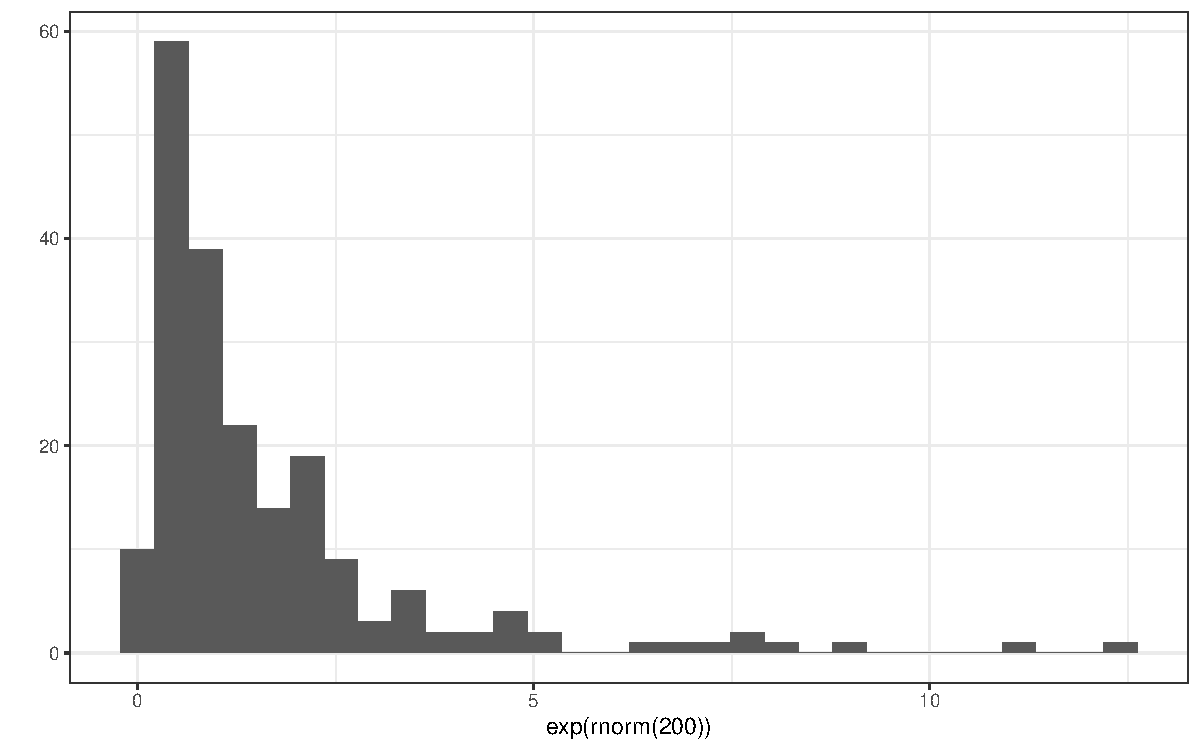
\includegraphics{examination_files/figure-latex/histogram-1.pdf}
\caption{\label{fig:histogram}Nice histogram.}
\end{figure}

\newpage
\printbibliography

\end{document}
